\begin{figure*}[t]
  \centering
  \begin{subfigure}[t]{0.24\linewidth}
    \centering
    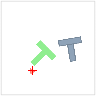
\includegraphics[width=\linewidth]{fig/render_robot.png}
    \caption{Robot domain (target)}
    \label{fig:teaser-robot}
  \end{subfigure}
  \hfill
  \begin{subfigure}[t]{0.24\linewidth}
    \centering
    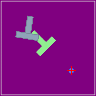
\includegraphics[width=\linewidth]{fig/render_human.png}
    \caption{Surrogate ego domain (source)}
    \label{fig:teaser-human}
  \end{subfigure}
  \hfill
  \begin{subfigure}[t]{0.47\linewidth}
    \centering
    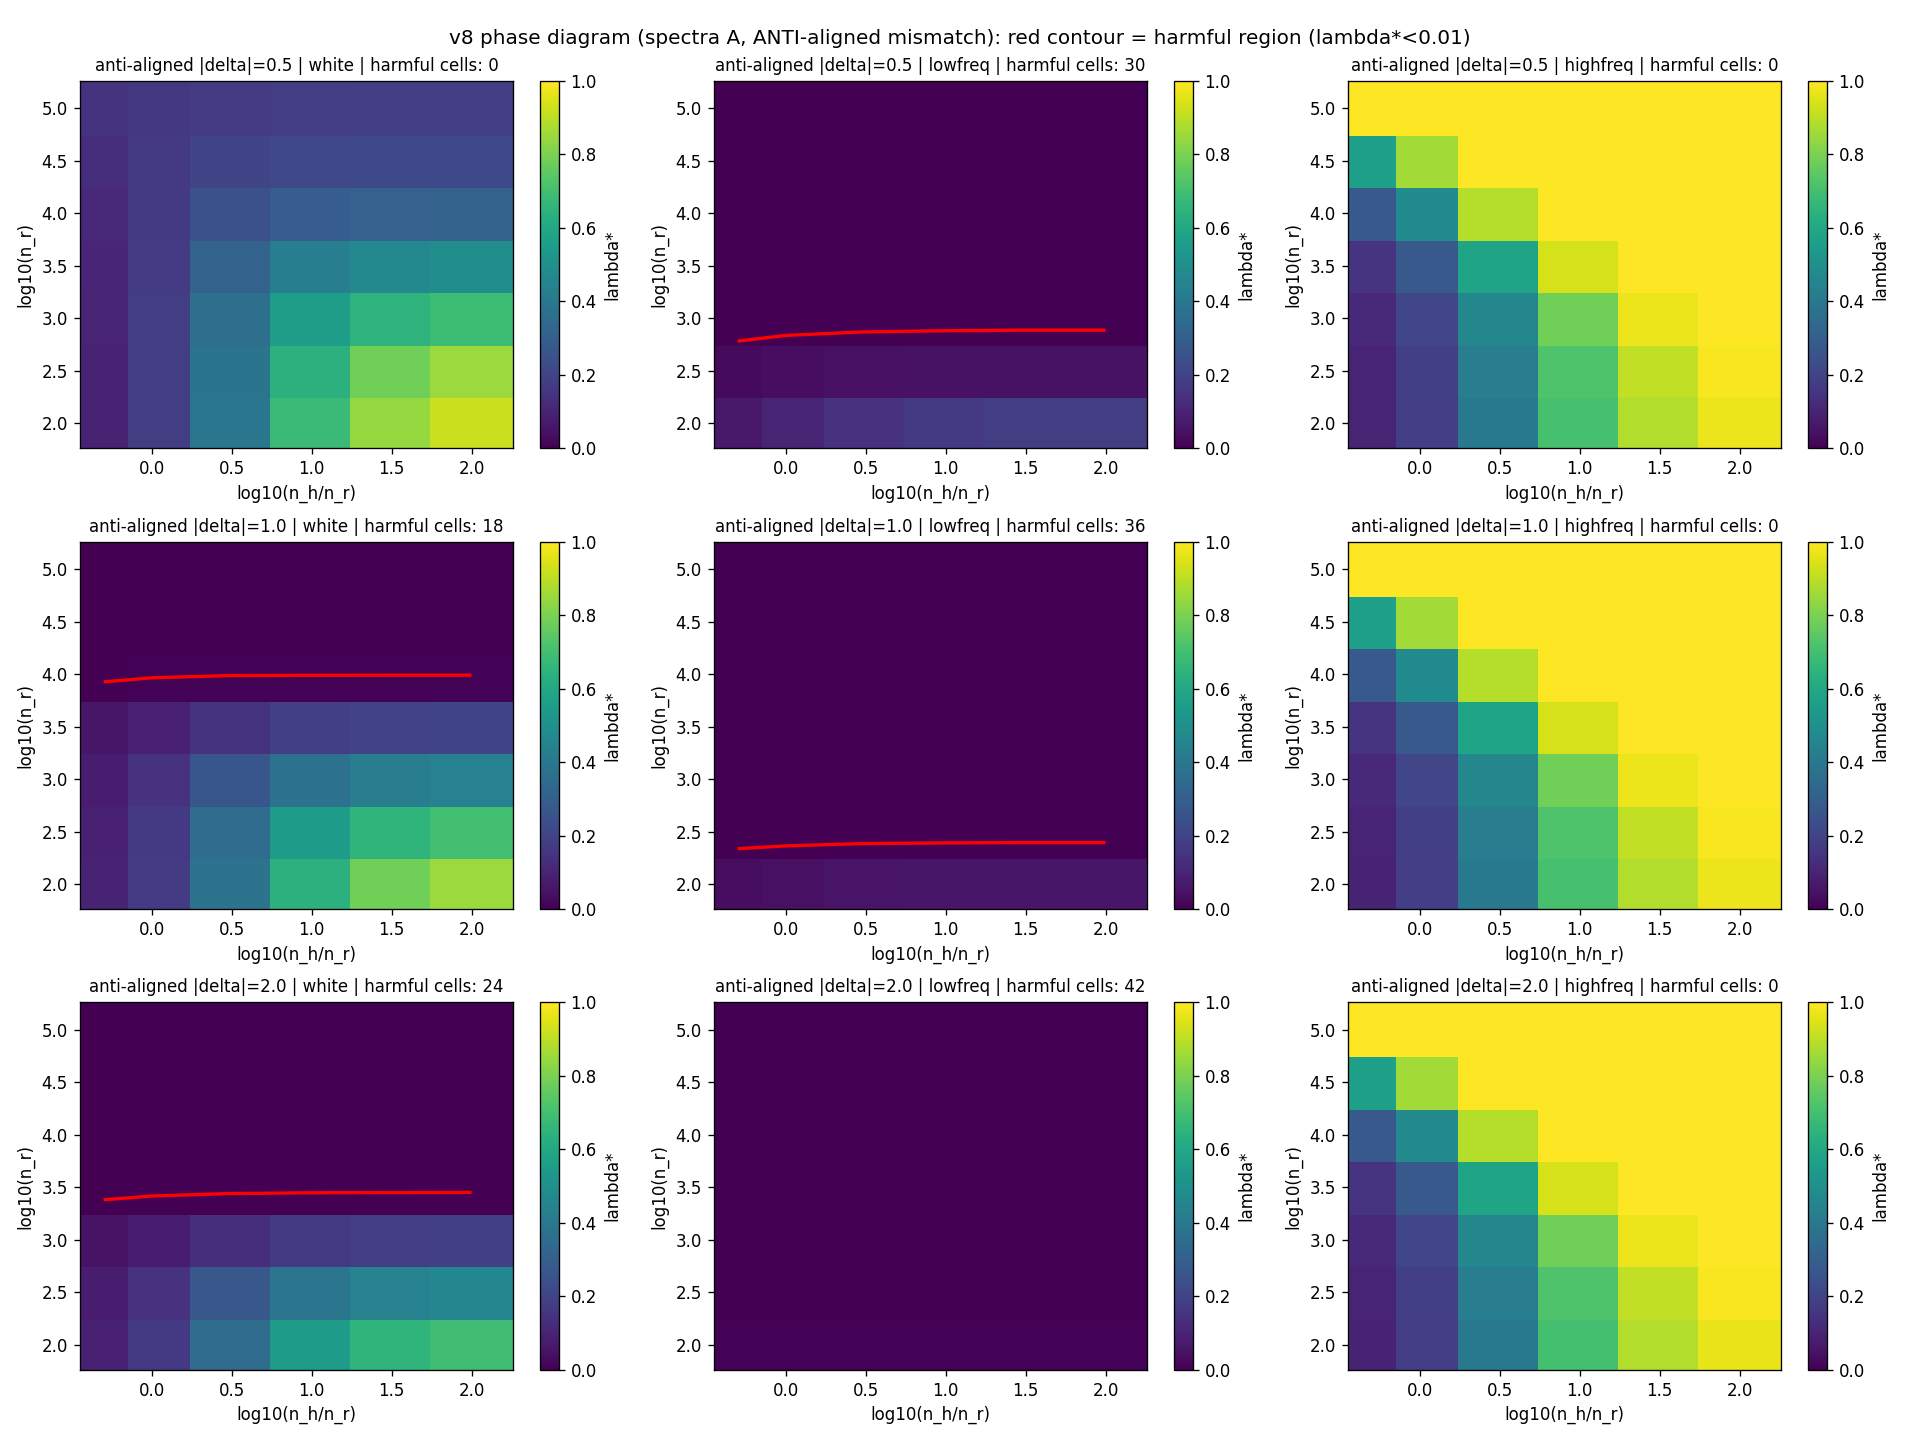
\includegraphics[width=\linewidth]{fig/phase_v8_anti.png}
    \caption{Theory: where mixing hurts}
    \label{fig:teaser-phase}
  \end{subfigure}
  \caption{\textbf{Cross-embodiment data mixing, modeled.}
  (a,b)~Our controlled dual-domain Push-T testbed pairs a robot domain with a surrogate egocentric-human domain that differs in appearance, actuator, friction, and task geometry (mirrored T-block configurations).
  (c)~The theory predicts \emph{where mixing hurts}: optimal mixing ratio $\lambda^*$ over the $(\nr,\, \nh/\nr)$ plane under anti-aligned mismatch; low-frequency-concentrated mismatch collapses $\lambda^*\!\to\!0$ (dark region), while the same mismatch energy placed on high-frequency coordinates is harmless everywhere (Sec.~\ref{sec:theory}).}
  \label{fig:teaser}
\end{figure*}
